\documentclass[convert={size=256}]{standalone}
\usepackage[utf8]{inputenc}
\usepackage[T1]{fontenc}
\usepackage{amsmath}
\usepackage{amssymb}
\usepackage{tikz}
\usepackage{color}

\definecolor{draculaPurple}{RGB}{189,147,249}
\definecolor{draculaCyan}{RGB}{139,233,253}
\definecolor{draculaForeground}{RGB}{248,248,248}

\begin{document}
	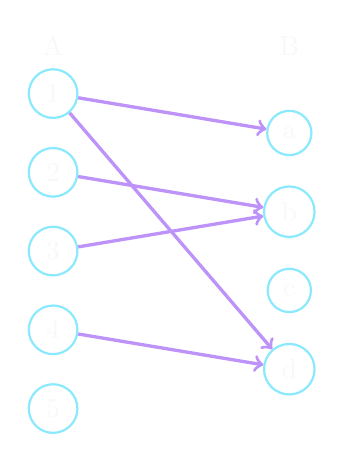
\begin{tikzpicture}[text=draculaForeground, draw=draculaCyan]
		\node at (0,-0.4) [thick] {A};
		\node at (3,-0.4) [thick] {B};
		\begin{scope}[every node/.style={circle,thick,draw}]
			\node (1) at (0,-1) {1};
			\node (2) at (0,-2) {2};
			\node (3) at (0,-3) {3};
			\node (4) at (0,-4) {4};
			\node (5) at (0,-5) {5};
		\end{scope}
		\begin{scope}[every node/.style={circle,thick,draw}]
			\node (A) at (3,-1.5) {a};
			\node (B) at (3,-2.5) {b};
			\node (C) at (3,-3.5) {c};
			\node (D) at (3,-4.5) {d};
		\end{scope}
		
		\begin{scope}[every edge/.style={draw=draculaPurple,very thick}]
			\path [->] (1) edge (A);
			\path [->] (1) edge (D);
			\path [->] (2) edge (B);
			\path [->] (3) edge (B);
			\path [->] (4) edge (D);
		\end{scope}
	\end{tikzpicture}
\end{document}